\chapter{Insufficiently related works}
These are outtakes from the related works chapter as they're insufficiently related to the core thesis to be included there. And yet, these topics are potentially relevant so could be re-included as needed in the main thesis or in future publications on related topics.


\section{Topics to include in the related works chapter}
The following hierarchical list includes topics I planed to include in the related works chapter. As they're here then at least some of them have been removed from that chapter :)


\begin{itemize}
    \item An overview on~\href{software.quality}{\emph{software quality}} including various viewpoints of quality e.g. Gerry Weinberg):
    \begin{itemize} 
        \item Nomenclature including multiple competing definitions of various NFRs. Mention ISO standards, \citep[Chapter 5]{chung2000_non_functional_requirements_in_software_engineering} on not prescribing relationships or the terms as their approach is intended to help the developers rather than dictate.
        \item Software defects, faults and failures~\hyperlink{defects.faults.failures}{\emph{link}}
        \item Bug investigation and localisation
        \item QoE: Quality of Experience
        \item Classic references e.g. Phadke~\citep{phadke1995_quality_engineering_using_robust_design} and perhaps Non-functional requirements in Software Engineering? 
        \item relevant / related academic research in my field
        \item Reliability. Introduced in ~\hyperlink{software.quality}{Software Quality}, and then expanded in a subsection~\hyperlink{software.reliability}{\emph{here}}
        \item Then focus on stability (as used by HP and then Google) encompassing reliability, freezes, etc.
        \item Discuss MTBF, usage paths and profiles and their effects on the measured values
        \item Maslow's hierarchy of needs where reliability is one of the base levels, yet vital. c.f Sommerville.
    \end{itemize}
    \item Measurement and Analytics
    \begin{itemize}
        \item Views from outside software engineering e.g. how to measure anything book
        \item Logging
        \item Telemetry
        \item Software Analytics e.g. Buse and Zimmermann
        \item Software Analytics tools and concepts e.g. free the data.
        \item Sources and mechanisms for collecting data and information about mobile apps
        \begin{itemize}
            \item Human-centric sources e.g. ratings and reviews. Perhaps also discuss some of the flaws and limitations either here or in the 'caveats...' section later?
            \item Perhaps also consider in-app feedback c.f. the Mobile Twin Peaks paper?
            \item Alpha, Beta, Crowd, and other forms of testing with subsets of a population.
            \item Program-centric sources e.g. logging, crash reporting libraries, analytics libraries, platform-level observations.
        \end{itemize}
        \item Using Data
        \item Privacy and Control
    \end{itemize}
    \item Software Development Practices
    \begin{itemize}
        \item Agile development and the effects on the software that is developed and released.
        \item Motivations for/of software developers.
    \end{itemize}
    \item Software Testing
    \begin{itemize}
        \item Schools of Software Testing? Old work that might help set the scene
        \item Classic references on software testing e.g. Boris Beizer
        \item using testing to measure quality and measuring software testing e.g. effectiveness.
    \end{itemize}
    \item App Stores and their effects on software development and engineering
    \begin{itemize}
        \item App Stores as ecosystems
        \item Release Planning (c.f DevOps and Release Engineering (including Shonan)
        \item Ratings and Reviews
        \item Google Play (and other Android app stores)
    \end{itemize}
    \item Developing mobile apps
    \begin{itemize}
        \item Single and multi-platform approaches
        \item A brief history of mobile app development
        \item Various species of bugs that affect mobile apps
    \end{itemize}
    \item Testing of Mobile Apps (this might be a distinct section in the Related Works as it's a rich topic). Do we care about testing of mobile apps that predates app store ecosystems?
    \begin{itemize}
        \item Automated testing frameworks and tools
        \item Testing practices (from both research and practical perspectives)
        \item Test Oracles
        \item Device Selection (as one aspect of testing for bug identification and investigation)
        \item Testing by crowds
        \item Measuring the efficacy of testing
    \end{itemize}
    \item Mobile Analytics~\hyperlink{mobile.analytics}{\emph{link}}
    \begin{itemize}
        \item types and sources of mobile analytics (also refer to appendix)
        \item Using Mobile Analytics to assess app behaviours
    \end{itemize}
    \item Caveats, constraints, flaws, limitations
    \begin{itemize}
        \item For instance on blind-spots, excessive trust and the ironies of automation. 
        \item Using crashes, ANRs, etc. as the test oracle - what will we miss if we only consider these aspects? how relevant is what we miss and what can we do to fill in some of the gaps?
    \end{itemize}
    \item Has anyone else published in my areas of research?
\end{itemize}

\section{App stores}
\textit{Generally, excluded from this topic: Windows, iOS, and BlackBerry ecosystems. Revenue generation such as in-app purchases, paid-for apps, advertising.} 

Dated works when BlackBerry and Windows Phone app stores existed. They mainly help set the context and identify there has been plenty of research into generations of the ecosystem but aren't sufficiently relevant to cover in the core thesis.

\section{In-app advertising}
While advertising in apps has been extensively researched the connection with mobile analytics is indirect. What they may share are:
\begin{itemize}
    \item Use of SDKs that have one of more libraries integrated into the app.
    \item Some form of tracking and reporting based on usage, however for advertising it's more likely to be tracking how many ads were served and the revenue the developer received rather than any other aspect of the app's behaviour or usage.
    \item Any adverse effects on the UX for end-users.
\end{itemize}


\section{Heatmapping}
User experience (UX) can be assessed using a wide variety of tools and techniques, such as heatmapping (which uses screen and/or interaction recording), A/B testing frameworks, funnel and journey analytics, and so on. By their very nature they're user-focused and - in practice - seldom incorporated into mobile apps or development practices for mobile apps. Similarly, based on my investigations, they are seldom researched although I have co-written work on this topic including examples of using heatmapping to improve usability of mobile apps~\cite{harty_aymer_playbook_2016}. Superficial research has been published to assess the events recorded by one of the heatmapping analytics tools - Appsee~\citep{yildirim2019_ux_analytics_for_android_platforms}. For those interested in developing a d-i-y approach to heatmapping there are a couple of options available including, the Caret-HM project~\footnote{\url{https://github.com/stlab-unt/Caret-HM}} that uses a web interface to interact with an Android emulator to record touchscreen interactions for apps installed on the emulator. The research is described in~\citep{nurmuradov2017_caret-hm-heatmapping-android-emulator}. It may be useful for small scale heatmapping however the combination of using a web interface with an emulator rather than actual Android devices limits the realism and the scale of the approach.

\section{Software Quality}

\subsection{Lived Experiences of testers using test-related tools}
\begin{figure}
    \centering
    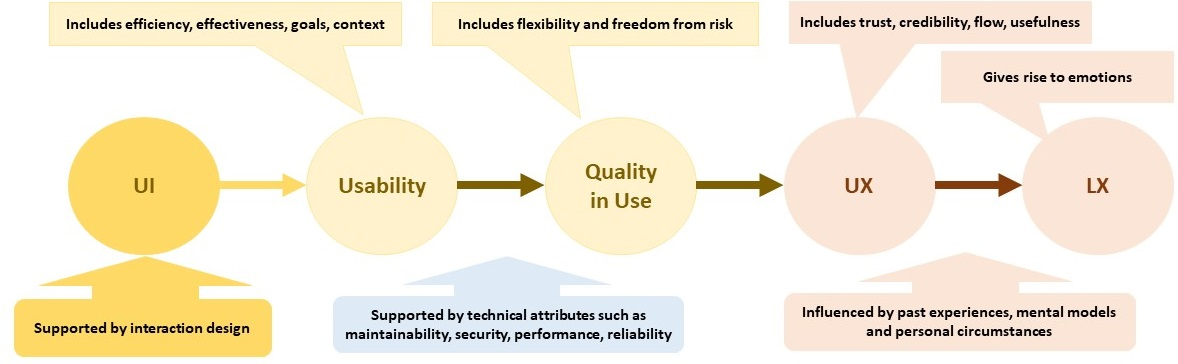
\includegraphics[width=15cm]{images/isabel-evans/Contributors_to_LX_v3.jpeg}
    \caption{Contributors to LX and Emotions, from~\citealp{evans2021_scared_frustrated_and_quietly_proud}}
    \label{fig:contributors-to-lx-and-emotions-v3}
\end{figure}

Figure \ref{fig:contributors-to-lx-and-emotions-v3}, from \citealp{evans2021_scared_frustrated_and_quietly_proud}, discusses factors that contribute to the lived experience of software testers using software tools. A similar consideration may extend these factors to the lived experiences of end users of mobile apps, and separately the lived experiences of users of mobile analytics tools?

%SHOULD-DO cover Quality of Experience (QoE) here. How users perceive QoE, how users communicate their QoE in an app store ecosystem, etc.


\section{Software development practices}
\subsection{Papers to consider on software development practices}
\begin{itemize}
    \item \emph{A systematic review of theory use in studies investigating the motivations of software engineers}~\citep{hall2009systematic}.
    \item \emph{Designing Engineering Onboarding for 60+ Nationalities}~\citep{harty2020_designing_engineering_onboarding}. Onboarding software developers and staff generally also includes exceptions and exception handling. These exceptions can be collected and analysed to determine where the onboarding is failing. Again there can be the concept of non-fatal and fatal exceptions. Fatal exceptions shouldn't happen ideally, there are mechanisms to handle them adequately in terms of error recovery, however we'd like to know about them and address them.
    \item \emph{Enabling Productive Software Development by Improving Information Flow}~\citep{murphy_enabling_2019}. 
    \begin{itemize}
        \item ``The flow of information among software developers is directly related to productivity."
        \item ``When the flow of information is adequately supported, delivery times on software can be shortened, and productivity within an organization can rise."
    \end{itemize}
    \item \emph{Continuous delivery sounds great, but will it work here?}~\citep{humble2018_continuous_delivery_sounds_great}. 
    \begin{itemize}
        \item ``Continuous delivery is about reducing the risk and transaction cost of taking changes from version control to production. Achieving this goal means implementing a series of patterns and practices that enable developers to create fast feedback loops and work in small batches. This, in turn, increases the quality of products, allows developers to react more rapidly to incidents and changing requirements and, in turn, build more stable and higher-quality products and services at lower costs."
        \item ``If this sounds too good to be true, bear in mind: continuous delivery is not magic. It's about continuous, daily improvement at all levels of the organization—the constant discipline of pursuing higher performance. As presented in this article, however, these ideas can be implemented in any domain; this requires thoroughgoing, disciplined, and ongoing work at all levels of the organization. Particularly hard, though essential, are the cultural and architectural changes required."
    \end{itemize}
    \item \emph{``One interesting line of future research is in estimating the maintenance cost for a mobile app. Currently there are just anecdotal estimates [3]."}~\citep[p. 27]{nagappan2016_future_trends_in_sw_eng_for_mobile_apps}. For additional information on reasons for lack of software maintenance in some app projects, see also, \emph{Mobile App Development and Management: Results from a Qualitative Investigation} in the excluded biography.
    
\end{itemize}


\section{Software Testing}

\subsection{Papers to consider}
\begin{itemize}
    \item TBC
    \item \emph{``Debugging without testing"}~\cite{ghardallou2016debugging_without_testing} It may be possible to demonstrate a bug has been fixed without testing, for instance by comparing behaviours before and after changes were made to the software. This paper's premise of being able to debug without testing held true in some of my research. Testing has not able to reproduce all the conditions needed for some bugs to emerge. Other information, such as stack traces, may help developers perceive likely causes of a bug, such as a crash, sufficiently for the developers to take what they believe is corrective action.  
    
    \item ~\emph{`Communication in Testing: Improvements for Testing Management'}~\citep{paakkonen2009_communication_in_testing}: 
    \begin{itemize}
        \item Three quality approaches: mapping of process, product, and quality-in-use => three perspectives: software engineer (developer), testing, and end-user. The first two are easier to measure for a software company, yet the quality-in-use is the most important for any product. \textbf{TBC}
    \end{itemize}
    
    \item Behaviourally Adequate Software Testing \url{https://leicester.figshare.com/articles/Behaviourally_Adequate_Software_Testing/10106189} - Behavioural Coverage, search-based white-box generation strategies. Measures of testing adequacy. \emph{One intuitive notion of adequacy, which has been discussed in theoretical terms over the past three decades, is the idea of behavioural coverage; if it is possible to infer an accurate model of a system from its test executions, then the test set must be adequate.} IIRC the programs they assess are tiny, and how can we determine 'accurate model', perhaps it'll be accurate for what it tests, but incomplete? "The truth, \emph{the whole truth}, and nothing but the truth" springs to mind. % See also Uncertainty-Driven Black-Box Test Data Generation (seems less relevant to my research) and Assessing Test Adequacy for Black-Box Systems Without Specifications (perhaps more relevant).
    
    \item Various papers listed on \url{https://testroots.org/publications.html} which focus on IDE measurements of developers running automated tests, CI and tests~\emph{``Oops, My Tests Broke the Build: An Explorative Analysis of Travis CI with GitHub"}, and code quality correlations between test and system code.
    
    \item "Probably approximately correct learning" however it seems to be unrealistic and impractical for shipping mobile app development teams.
\end{itemize}


\subsection{Record and Playback - extends logging for various purposes}
\newthought{Record and replay/playback}
Recreate the `journey' (however relevant context may be missing or different and therefore affect the results and conclusions). Various reasons why recreating the journey is desirable e.g. to reproduce failures to help understand their characteristics and causes, to learn indirectly by observing and visualising the journey. \emph{c.f.} heatmapping. Record and replay offers the possibility of moving beyond using breadcrumbs as it is intended to record sufficient information to reproduce the use of an app. However there are various limitations in the tooling, the techniques, and at least as importantly the unacceptability of recording end user sessions on their devices using production releases of apps downloaded from the app store. 

\newthought{Prior art in record and replay/playback}
TBC

\hypertarget{mobile.testing}{}
\section{Testing Mobile Apps}

There has been a tremendous amount of research into practices and tools that might perform better than the mainstream test automation tools available to app developers.

A useful categorisation of testing for mobile apps may be: 
explicitly designed scripted tests, 
automatic robots that navigate and sometimes interrogate target apps, and 
hands-on testing which often vary depending on who performs them and each instance of the testing. 
Where the testing may be performed:
on local physical devices,
on remote physical devices in the `cloud'
on local emulators and/or local simulators, and
on remote emulators and/or simulators.



\subsection{Papers to consider}
\begin{itemize}
    \item \emph{``To the attention of mobile software developers: guess what, test your app!"}~\citep{cruz2019_guess_what_test_your_app}.
    
    \item Discuss the TestDroid paper! it describes testing that was actually done by developers!~\citet{kaasila2012_testdroid_etc}.
    
    \item \emph{``PRADA: Prioritizing Android Devices for Apps by Mining Large-Scale Usage Data"}~\citep{lu2016_PRADA}. 
        
    \item \emph{``Automatically Discovering, Reporting and Reproducing Android Application Crashes"}~\citep{moran2016_automatically_drr_android_app_crashes}.
    
    \item \emph{``Is Mutation Analysis Effective at Testing Android Apps?"}~\citep{deng2017_is_mutation_analysis_effective_at_testing_android_apps}.
    
    \item \emph{``Mining Android Crash Fixes in the Absence of Issue- and Change-Tracking Systems"}~\citep{kong2019_mining_android_crash_fixes}.
    
    \item \emph{``How do Developers Test Android Applications?"}~\citep{linares2017_how_do_developers_test_android_apps}. Quote:~\emph{``“I mostly do manual testing due to the limited size of my apps. I sometimes use a custom replay system (built into the app) to duplicate bugs after I come across them. This method is usually combined with manual testing (printing debug information to the log) to pinpoint the cause”."}
    
    \item \emph{``Prioritizing the Devices to Test Your App on: A Case Study of Android Game Apps"}~\citep{khalid2014_prioritizing_the_devices_to_test_your_app_on_casestudy_android_games}.
    
    \item \emph{``First Steps in Retrofitting a Versatile Software Testing Infrastructure to Android"}~\citep{oliver2018_first_steps_in_retrofitting_a_versatile_sw_testing_architecture}.
    
    \item \emph{``A Large-Scale Study of Application Incompatibilities in Android"}~\citep{cai2019_large_scale_study_of_android_incompatibilities} An oddly insipid paper which promised some interesting run-time issues discovered in their research where the Android version would be a likely cause. However the reproduction package lacked the test scripts or means to reproduce their testing or bug detection. Also, their research now seems to be less relevant in 2020 as Android apparently improved the backwards compatibility \emph{``Yet newer versions (since API 24) had no run-time compatibility issues with apps created in the studied span."}. Their work may well have merit for the research community, It does not appear to have much relevance to developers of real-world Android apps today.
    
    \item \emph{`A Case Study of Automating User Experience-Oriented Performance Testing on Smartphones"}~\citep{canfora2013_automating_UX_experience_testing_on_smartphones}. %30 citations in Google Scholar. 
    This research focused on whether their ATE (Automated Testing Equipment) could detect and score perceived UX of two versions of an Android phone, the HTC~\textsuperscript{\textregistered} Nexus One. The key difference was a reduction of RAM by 30\% which made their simple Android application slower on the version with less RAM. They used and processed Android logs to record the differences in timing information. Their ATE provided similar quality scores to human volunteers who used both versions of the phone. Their ATE equipment incorporated servo motors to move the phone around on an otherwise fixed testbed and a camera to record the GUI. (Curiously their photo shows they were using a Samsung phone rather than the one described in the paper.) The paper lacked details of the hardware, the movements the servos provided, or of the simple Android application they created and used for their evaluation.
    Note: Their approach in moving the phones appears similar to that used by LessPainful (a now defunct company, since acquired ultimately by Microsoft) who provided a commercial testing service across a wide range of Android \textit{and} iOS devices. 
    This paper's work is relevant for its use of Android logs and logging to record and analyse the usage of the device. Unfortunately there appear to be several material flaws in the paper, for example where they state: ~\emph{`...a score of 30 for CUST-37..."} the only mention of CUST-37 whereas the rest of the paper refers to a CUST-30 configuration (with 30\% less RAM). Have they transposed the two numbers ~\emph{e.g.} should it be a score of 37 for CUST-30? and on a related note, their calculation of the percentage difference in their ATE generated UX score says the CUST-30 received a score of 4.05/5 while the stock configuration received a score of 4.54/5. While the difference in the scores by the humans of 4.54/4.05 is approximately 12\% these scores are out of 5, so the percentage should be twice the one they used ~\emph{i.e. approximately 22.42\%}  \texttt{=((4.54/4.05)/5.00)*100\%}.
    
    \item \emph{``Intent Fuzzer: Crafting Intents of Death"}~\citep{10.1145/2632168.2632169} TODO Link this to the industrial case study and the Kotlin NPE crash.
    
    \item \emph{`A Grey-Box Approach for Automated GUI-Model Generation of Mobile Applications'}~\citep{Yang_Prasad_Xie_2013_grey_box_automated_gui_model_generation_for_mobile_apps}: This is one of the relatively early papers that focused on model-based testing for mobile apps. They used a simpilified version of a simple tip calculation app as their example application under test. They further similify the complexity by ignoring changes in the application state related to different data values. Their work built on the work of various approaches to `crawling' GUIs of an application and provides one of the roots of automated dynamic interactions with fairly simple opensource Android applications. It achieved good coverage for these apps. Through no fault of their research mobile apps, and particularly successful mobile apps are far removed from the apps they tested and their approach and tool has fallen into disuse. %Nonetheless two of the authors were granted a US patent for their approach in 2019! :( Automatically extracting a model for the behavior of a mobile application. MR Prasad, W Yang - US Patent 10,360,027, 2019
    
    \item "Mobile Testing-as-a-Service (MTaaS)--Infrastructures, Issues, Solutions and Needs"~\cite{gao2014mobile}. This paper, published in 2014, in my view isn't particularly novel. Rather it summed up stuff that was happening in industry at the time and combined it with a bunch of ideas of what \emph{might} be worth doing in the authors' view. The aim of the authors is to set the direction for scaling testing of mobile apps. Six years on is a good time to assess their suggestions.
    
    \item "The Testing Method Based on Image Analysis for Automated Detection of UI Defects Intended for Mobile Applications". \textbf{Springer paper I paid for.}
    
    \item \emph{``Linares-Vasquez et al. [56] propose MonkeyLab, which mines recorded executions to guide the testing of Android mobile apps."} Their approach records GUI events (click events). Members of the project team (developers, testers, etc.) perform the actions, the authors claim their log collection process could scale to collecting logs from ordinary users. Key limitations include events that aren't purely dependent on the user's GUI inputs, there would also be challenges getting users to accept such an approach where the app records every input they made. Also, they generate GUI events that have x,y coordinates - absolute positioning that may have limited portability to other devices, screen rotations, and so on. Their playback also appears to require rooted devices. There are numerous other limitations described in their paper, nonetheless their work shows promise in terms of detecting and generating patterns the students did not find. It would be interesting to compare the results using accomplished software testers with experience and expertise testing similar Android apps.
\end{itemize}

There has been a tremendous and sustained research interest in software testing, for instance testing is one of the most popular topics at the ICSE series of conferences~\footnote{\url{https://dl.acm.org/conference/icse}} and the focus of entire conferences including AST~\footnote{\url{https://conf.researchr.org/home/icse-2020/ast-2020}}, ICST~\footnote{\url{https://conf.researchr.org/series/icst}}, and so on. Similarly the application of software testing to mobile apps is a rich topic with sustained interest in the challenges and facets of testing mobile apps.

The facets include automated testing and automated bug reproduction, maximising the `bang for the buck' for instance in selecting which device models would be most valuable to use with finite testing. Understandably given the field where many of the authors work - in research - the vast majority of the research is on software apps they have access to, software their can obtain the source code for (particularly opensource), software they can write, and the people they have available to them (other researchers, students, voluntary participants, and people paid to paid to perform specific tasks). Minute amounts of the work is based on mature, popular software with semi- or fully- professional developers and development teams. Some research projects, particularly CRASHSCOPE~\citep{moran2016_automatically_drr_android_app_crashes}, offer the potential to reproduce some of the crashes reported by Mobile Analytics if the tools are sufficiently available and current to actually use.



There is some interesting large-scale research into analysis of various releases of production Android application binaries~\citep{kong2019_mining_android_crash_fixes}. The researchers exercised (tested) a large range of apps seeking crashes of the app using an oracle of a local log file which they queried using the standard Android \texttt{logcat} utility. They also combined their dynamic approach with using static analysis tools to identify potential flaws that would lead to crashes of an app. They then tested newer releases of the same app. If the newer version did not crash they analysed the binary files (the APK files) for both releases to differences to the compiled code that may have been responsible for 'fixing' the crash. They limited their work to Android \emph{framework specific} crashes, and excluded \emph{app-specific} crashes. They devised ways to identify changes that appeared to fix the particular crash(es) they triggered in the earlier releases and generated patch files based on these changes. These patches were then applied to the older release of the app and the app then tested with the same test inputs and runtime environment (at least in terms of using a consistent Android Emulator (also known as a virtual device)). They provide a relatively detailed replication package online at~\url{https://craftdroid.github.io/}.

\begin{itemize}
    \item Their approach is innovative and could help real-world developers of Android apps to identify and apply snippets of code to reduce the likelihood of their app suffering the same crash. Their 17~\href{https://github.com/CraftDroid/ExpData/tree/master/Fix_Templates}{fix templates} act as guides for Android developers and could potentially be implemented into code-quality tools.
    \item However it only applied for framework specific crashes, and their choice of runtime environment meant they could only install 56\% of the APKs. There are many other sources of crashes, and also apps that include native code (several of my case study apps do). Also their testing is limited to automated `monkey' testing which may further limit the crashes their approach can find in production apps, particularly those that incorporate user accounts, user-specific content, behaviour, online purchases and many other forms of activities.
    \item The supporting website \url{https://github.com/CraftDroid} includes scripts and log extracts for the crash reproductions, it lacks the mechanisms for generating diffs, applying them, or building the patched APK. The lack of these mechanisms makes the efficacy of their approach hard to reproduce.
    \item It also does not appear to test for crashes related to third-party libraries e.g. OkHttp which is extremely popular in Android apps; however potentially this approach could be extended to do so?
\end{itemize}

In summary, the approach proposed in~\citep{kong2019_mining_android_crash_fixes} has the potential to mine crash stack traces (which are available to the developers of the particular apps) to help with aspects of reproducing a subset of those crashes which pertain to Android framework-related crashes. Similarly it appears it could complement the automated testing provided by Google as part of the pre-launch reports available in Google Play Console and other services. 

\subsection{Prioritising devices to test on}

Selection criteria include:
\begin{itemize}
    \item the relative popularity of a single app across the user base for the app, provided by OpenSignal, and reported over a three year period,
    \item the usage of similar, popular, Android apps for two app categories: grouped by device model as measured by a very popular app management app in China,
    \item the devices used most frequently by users who write reviews for the same Android app,
\end{itemize}

One of the research papers close to the area of my research uses usage data for two popular app categories (games and media) gathered through a popular Android management app in China~\citep{lu2016_PRADA}. Their work uses an operational profile to prioritise the device models to select to test both new or existing apps. The management app, called Wandoujia~\footnote{\url{https://www.wandoujia.com/}}, is used by \emph{`500 million people to find apps they want`}~\footnote{According to Chrome Browser's automatic translation from Chinese.}. Daily usage of the top 100 apps in the two app categories was collected for various device models. In various ways the Wandoujia app management app provides similar capabilities to Google Play, including tracking when apps are installed, and in use. The recommendations are coarse-grained. The research measured the accuracy of their predictions for recommended devices with the actual devices that the app ended up being used on once the app had been launched. 

Their work demonstrates that usage data for several app categories was useful to guide developers on the most popular actual device models for their app. They acknowledge several limitations in their work, including their use of incomplete measures such as foreground network activity for usage which don't suit apps that either perform network processing in the background or don't use the network. Other app management services, particularly Google Play, could provide similar guidance to app developers. And indeed as Google Play collects additional data for the entire apps store it could cover some of the gaps and limitations identified in this research.


\subsubsection{Device Testing Services}
Test Farms have been available commercially since around 2008~\footnote{Based on the author's professional experience.}. Over the years different offerings have peaked and then either been acquired, retired, or disappeared. Google, Amazon and Microsoft offer paid-for device farms as do various specialist businesses. There have been a couple of public-good initiatives including Open Device Labs~\footnote{For example~\url{https://opendevicelab.com/},~\url{https://www.devicelab.org/}}; and Open STF~\cite{openstf_website} which is based on a set of opensource projects~\url{https://github.com/openstf/} and enables teams and organisations to build their own device farms or use commercial offerings based on these projects~\footnote{For example~\url{https://www.headspin.io/}.}.
% https://loadfocus.com/blog/tech/2018/04/building-your-in-house-device-farm-on-mac-os-using-openstf-for-android-testing/ 
% https://tech.mercari.com/entry/2019/02/18/173236 (on using HeadSpin and NimbleDroid).


\section{Software Testing}
Here are the key papers in terms of this research from the incredibly rich variety of papers on software testing generally and software testing for mobile apps in particular. I cannot hope to do justice to the entire topic in the context of a PhD on mobile analytics.

From the perspective of app developers software testing they appreciate obtaining sufficient confidence the app will function adequately and that recent changes to the codebase have not broken in predictable areas. 


\subsection{Papers to consider}
\begin{itemize}
    \item TBC
    \item \emph{``Debugging without testing"}~\cite{ghardallou2016debugging_without_testing} It may be possible to demonstrate a bug has been fixed without testing, for instance by comparing behaviours before and after changes were made to the software. This paper's premise of being able to debug without testing held true in some of my research. Testing has not able to reproduce all the conditions needed for some bugs to emerge. Other information, such as stack traces, may help developers perceive likely causes of a bug, such as a crash, sufficiently for the developers to take what they believe is corrective action.  
    
    \item ~\emph{`Communication in Testing: Improvements for Testing Management'}~\citep{paakkonen2009_communication_in_testing}: 
    \begin{itemize}
        \item Three quality approaches: mapping of process, product, and quality-in-use => three perspectives: software engineer (developer), testing, and end-user. The first two are easier to measure for a software company, yet the quality-in-use is the most important for any product. \textbf{TBC}
    \end{itemize}
    
    \item Behaviourally Adequate Software Testing \url{https://leicester.figshare.com/articles/Behaviourally_Adequate_Software_Testing/10106189} - Behavioural Coverage, search-based white-box generation strategies. Measures of testing adequacy. \emph{One intuitive notion of adequacy, which has been discussed in theoretical terms over the past three decades, is the idea of behavioural coverage; if it is possible to infer an accurate model of a system from its test executions, then the test set must be adequate.} IIRC the programs they assess are tiny, and how can we determine 'accurate model', perhaps it'll be accurate for what it tests, but incomplete? "The truth, \emph{the whole truth}, and nothing but the truth" springs to mind. % See also Uncertainty-Driven Black-Box Test Data Generation (seems less relevant to my research) and Assessing Test Adequacy for Black-Box Systems Without Specifications (perhaps more relevant).

\end{itemize}


\subsection{Concepts to consider}
\begin{itemize}
    \item Adequacy
    \item Confidence levels (in the testing we've done)
    \item Sufficiency (c.f. how Google graded OKRs where 0.7 was the expected, sufficient, amount of progress).
    \item What testing actually gets done for real software, rather than what testing standards, academia, etc. tells us we \emph{should} do.
    \item Probably Approximately Correct.
    \item Testing logging and analytics, especially when many aspects of the systems are provided by third-parties, involves determining causal links between two phenomena. Concommitant variations, introduced in~\cite{mill1884system}
    \item Who tests the software developers use? for instance the many APIs and libraries? Flaws in this software, created by others, may affect the development teams and the users of their software products, amongst others. This software will include proprietary code and will probably include opensource code, perhaps pre-packaged as libraries of binary code. Some of that software may be poorly maintained, and yet the quality of that software may adversely affect the quality of the code using it. 
\end{itemize}



\subsection{Bugs}
Species of bugs: inadequate and neglected error handling, data loss bugs.

Exception handling is strongly related to program robustness.~\citep{Oliveira_Borges_Silva_Cacho_Castor_2018_android_error_handling}. In particular, they observed that developers did not write sufficient code to handle exceptions that could be thrown when their Android app uses Android-specific abstractions. Uncaught exceptions lead to the application crashing, and crashes are an indication of poor reliability of the application. Of course, the exception needs to occur in order for the app to crash, and not every uncaught exception causes the app to crash, they may crash an internal thread within the app instead~\citep{Oliveira_Borges_Silva_Cacho_Castor_2018_android_error_handling}. %Note: not all caught exceptions are handled adequately. E.g. some may simply be logged and the code allowed to continue unchanged. Sometimes the exception may mean internal state and/or data are incomplete or incorrect for reliable and correct operations of the app. 
Their research excluded various factors that also affect robustness, in particular they chose not to study: ``security vulnerabilities, excessive resource consumption, and race conditions."~\citep{Oliveira_Borges_Silva_Cacho_Castor_2018_android_error_handling}. %As an observation, they appear to over-state the LOC they analysed, or at least they're inflating the counts to count every line of code six-times even if those lines are identical for two or more releases.

In the work of~\citep{khalid2015_what_do_mobile_app_users_complain_about} the authors note that iOS apps with frequent functional errors or crashes are more likely to be rated poorly in the app store. Their work did not extend to Android apps, however it seems reasonable that errors and crashes in Android apps would also lead to lower ratings in the app store, and conversely Google states that~\emph{``Performance and stability are directly linked to positive ratings on Google Play."}~\citep{android_vitals_best_practices}.

\textbf{MUST-DO} write about the fault-proneness paper reference on Android APIs: one source that causes crashes is the revision of APIs used by Android apps~\citep{linares2013_api_change_and_fault_proneness_android}.
% via Oliveria... 
% Linares-Vásquez et al. (2013) investigated the relation between the success of Android applications (in terms of user ratings) and the change- and fault-proneness of the underlying APIs. They have computed bug fixes and changes in the interfaces, implementation and exception handling of 7.097 Android applications belonging to different domains. They found that APIs used by successful apps (high user ratings) are significantly less change- and fault-proneness than APIs used by unsuccessful apps. In terms of changes to the set of exceptions thrown by methods, the study did not observe any significant difference between different levels of rating.

% via Oliveria...
% Bhattacharya et al. (2013) performed an in-depth empirical study on bugs in 24 widely-used open-source Android apps from diverse categories such as communication, tools, and media. They sought to understand the nature of bugs and bug-fixing processes associated with smartphone platforms and apps. They defined several metrics to analyze the bug fixing process. They showed how differences in bug life-cycles can affect the bug fixing process and performed a study of Android security bugs. 

\emph{``Characterizing Android-Specific Crash Bugs"}~\citep{jha2019_characterizing_android_specific_crash_bugs} TBC.


Data loss bugs: When apps lose data they also lose the trust of users. One cause of data loss in Android apps has been investigated recently (2019) in ~\cite{riganelli2019benchmark_android_data_loss_bugs} where the authors found 19.2\% of the Android apps they evaluated lost data. The data losses were of one particular type - where the app failed to save and/or restore data when the app was stopped and restarted. There are other causes of data loss for mobile apps including database, network and storage errors, for example. They claim some of these bugs may surface as crashes in the app at a later stage, after the data was lost and the app resumed, however their examples did not seem to result in crashes. \yijun{Data loss is definitely a sign of lack of integrity. Sometimes it is required to lose some user data for privacy protection. Maybe you can refine the definitely more precisely to refer to "retaining the data that users care".} \yijun{I think one of the gaps is that the data loss bug that does not lead to crashes are actually bugs too. This is kind of important to justify your work will be different from other app testing literature that focus on detecting crash related bugs.}

To the authors' credit they provide extensive material including automated tests for the vast majority of the bugs~\footnote{\url{https://gitlab.com/learnERC/DataLossRepository}}. They were able to create automated tests that reproduced 110 of the 116 errors and were able to automatically detect 98 out of the 110 errors they were able to reproduce.

One of the considerations this work helps to illustrate is the many challenges of measuring software quality comprehensively, or even adequately.

\newthought{Taming Android App Crashes}
Given there are bugs that lead to crashes in mobile apps, are there ways to reduce the volume and/or impact of the crashes? MUST-DO work through the papers found using the following search:~\url{https://scholar.google.com/scholar?hl=en&q=Taming+Android+App+Crashes&btnG=&oq=jeff+off}


\textbf{TODO} Wrap up this sub-section with where most of the research has been in terms of bugs in mobile apps.


